\documentclass{article}

\usepackage{fancyhdr}
\usepackage{lastpage}
\usepackage{extramarks}
\usepackage[usenames,dvipsnames]{color}
\usepackage{amsmath}
\usepackage{amsthm}
\usepackage{amsfonts}
\usepackage{changepage}
\usepackage{lineno}
\usepackage[plain]{algorithm}
\usepackage{algpseudocode}
\usepackage{hyperref}
\usepackage{tikz}

\topmargin=-0.45in
\evensidemargin=0in
\oddsidemargin=0in
\textwidth=6.5in
\textheight=9.0in
\headsep=0.25in

\linespread{1.1}

\pagestyle{fancy}
\lhead{\hmwkAuthorName}
\chead{\hmwkClass\ (\hmwkClassInstructor\ \hmwkClassTime): \hmwkTitle}
\rhead{\firstxmark}
\lfoot{\lastxmark}
\cfoot{}

\renewcommand\headrulewidth{0.4pt}
\renewcommand\footrulewidth{0.4pt}

\setlength{\floatsep}{100pt}
\renewcommand{\algorithmicrequire}{\textbf{Input:}}
\renewcommand{\algorithmicensure}{\textbf{Output:}}
\algrenewcomment[1]{\hfill // #1}

\setlength\parindent{0pt}

\hypersetup{colorlinks=true}

\newcommand{\enterProblemHeader}[1]{
    \nobreak\extramarks{}{Problem \arabic{#1} continued on next page\ldots}\nobreak{}
    \nobreak\extramarks{Problem \arabic{#1} (continued)}{Problem \arabic{#1} continued on next page\ldots}\nobreak{}
}

\newcommand{\exitProblemHeader}[1]{
    \nobreak\extramarks{Problem \arabic{#1} (continued)}{Problem \arabic{#1} continued on next page\ldots}\nobreak{}
    \stepcounter{#1}
    \nobreak\extramarks{Problem \arabic{#1}}{}\nobreak{}
}

\setcounter{secnumdepth}{0}
\newcounter{partCounter}
\newcounter{homeworkProblemCounter}
\setcounter{homeworkProblemCounter}{1}
\nobreak\extramarks{Problem \arabic{homeworkProblemCounter}}{}\nobreak{}

\newenvironment{homeworkProblem}{
    \section{Problem \arabic{homeworkProblemCounter}}
    \setcounter{partCounter}{1}
    \enterProblemHeader{homeworkProblemCounter}
}{
    \exitProblemHeader{homeworkProblemCounter}
}

\newcommand{\hmwkTitle}{Homework\ \#1}
\newcommand{\hmwkDueDate}{January 22, 2014}
\newcommand{\hmwkClass}{Stat330}
\newcommand{\hmwkClassTime}{Section A}
\newcommand{\hmwkClassInstructor}{Mr. Lanker}
\newcommand{\hmwkAuthorName}{Josh Davis}

\title{
    \vspace{2in}
    \textmd{\textbf{\hmwkClass:\ \hmwkTitle}}\\
    \normalsize\vspace{0.1in}\small{Due\ on\ \hmwkDueDate at 3:10pm}\\
    \vspace{0.1in}\large{\textit{\hmwkClassInstructor\ \hmwkClassTime}}
    \vspace{3in}
}

\author{\textbf{\hmwkAuthorName}}
\date{}

\newcommand{\alg}[1]{\textsc{\bfseries \footnotesize #1}}
\newcommand{\deriv}[1]{\frac{\mathrm{d}}{\mathrm{d}x} (#1)}
\newcommand{\dx}{\mathrm{d}x}
\newcommand{\solution}{\textbf{\large Solution}}

\renewcommand{\part}[1]{\textbf{\large Part \Alph{partCounter}}\stepcounter{partCounter}\\}


\begin{document}

\maketitle

\pagebreak


\begin{homeworkProblem}
    Math and calculus review.
    \\

    \part

    Evaluate \(\sum_{k=1}^{5} k^2\) and \(\sum_{k=1}^{5} (k - 1)^2\).
    \\

    \solution

    \[
        \begin{split}
            \sum_{k=1}^{5} k^2 = 1^2 + 2^2 + 3^2 + 4^2 + 5^2 = 55
        \end{split}
    \]
    \[
        \begin{split}
            \sum_{k=1}^{5} (k - 1)^2
            &= (1 - 1)^2 + (2 - 1) ^2 + (3 - 1)^2 + (4 - 1)^2 + (5 - 1)^2 = 30
        \end{split}
    \]
    \\

    \part

    Find the derivative of \(f(x) = x^4 + 3x^2 - 2\)
    \\

    \solution

    \[
        \deriv{x^4 + 3x^2 - 2}
        = 4x^3 + 6x
    \]
    \\

    \part

    Find the derivative of \(f(x) = 1 - \mathrm{e}^{-\lambda x}\).
    \\

    \solution

    \[
        \deriv{1 - \mathrm{e}^{-\lambda x}}
        = \lambda \cdot \mathrm{e}^{- \lambda x}
    \]
    \\

    \part

    Evaluate the integrals \(\int_0^1 (1 - x^2) \dx\) and \(\int_1^{\infty} \frac{1}{x^2} \dx\).
    \\

    \solution

    \[
        \int_0^1 (1 - x^2) \dx
        = \left. x - \frac{1}{3}x^3 \right|_0^1
        = (1 - \frac{1}{3}) - (0 - 0)
        = \frac{2}{3}
    \]

    \[
        \begin{split}
            \int_1^\infty \frac{1}{x^2} \dx
            &= \lim_{b \to \infty} \int_1^b \frac{1}{x^2} \dx
            \\
            &= \lim_{b \to \infty} \left. - \frac{1}{x} \right|_1^b
            \\
            &= \lim_{b \to \infty} - \frac{1}{b} + \frac{1}{1}
            \\
            &= 1
        \end{split}
    \]
\end{homeworkProblem}

\pagebreak

\begin{homeworkProblem}
    Examples of sample spaces.
    \\

    \part

    Driving to work and passing through 3 intersections.
    \\

    \solution

    \[
        \Omega =  \left\{ ccc, ccs, csc, css, scc, scs, ssc, sss  \right\}
    \]
    \\

    \part

    What is the probability that she doesn't stop?

    \[
        \Pr(\mbox{no stops}) = \frac{\left| \left\{ ccc \right\} \right| }{\left| \Omega \right|} = \frac{1}{8}
    \]
    \\

    \part

    Let \(A\) be the event that the commuter stops at the first light. Let
    \(B\) be the event that the commuter stops at the second light.
    \\

    \solution

    \begin{enumerate}
        \item \(A = \left\{ scc, scs, ssc, sss \right\}\)
        \item \(B = \left\{ csc, css, ssc, sss \right\}\)
        \item \(\overline{B} = \left\{ ccc, ccs, scc, scs \right\}\)
        \item \(A \cup B = \left\{ scc, scs, csc, css, ssc, sss \right\}\)
        \item \(A \cap B = \left\{ ssc, sss \right\}\)
        \item \(A \cap \overline{B} = \left\{ scc, scs \right\}\)
    \end{enumerate}

\end{homeworkProblem}

\pagebreak

\begin{homeworkProblem}
    Let \(G\) and \(H\) be disjoint events in some sample space \(\Omega\).
    \\

    \part

    Describe the event \(G \cup H\).
    \\

    \solution

    A new event that includes outcomes in \(G\) \textbf{or} in \(H\).
    \\

    \part

    What is \(P(G \cup H)\) in terms of \(P(G)\) and \(P(H)\)?
    \\

    \solution

    Since \(G\) and \(H\) are disjoint, \(P(G \cap H) = 0\):

    \[
        \begin{split}
            P(G \cup H) &= P(G) + P(H) - P(G \cap H)
            \\
            &= P(G) + P(H) - 0
            \\
            &= P(G) + P(H)
        \end{split}
    \]
    \\

    \part

    Describe the event \(G \cap H\).
    \\

    \solution

    A new event that includes the outcomes that happen in event
    \(G\) \textbf{and} in \(H\).
    \\

    \part

    What is the probability of event \(G \cap H\)?
    \\

    \solution

    The probability of \(G \cap H = 0\) because the two events are disjoint.
\end{homeworkProblem}

\pagebreak

\begin{homeworkProblem}
    Venn diagrams. The grey areas indicate the solution.
    \\

    \part

    \(A \cup B\)
    \\

    \solution

    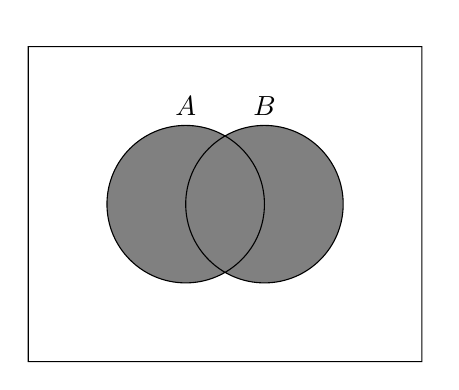
\begin{tikzpicture}[fill=gray]
        \begin{scope}
            \fill (0,0) circle (1);
            \fill (1,0) circle (1);
        \end{scope}

        \draw (0,0) circle (1) (0,1)  node [text=black,above] {$A$}
              (1,0) circle (1) (1,1)  node [text=black,above] {$B$}
              (-2,-2) rectangle (3,2) node [text=black,above] {};
    \end{tikzpicture}

    \part

    \(\overline{A \cup B}\)
    \\

    \solution

    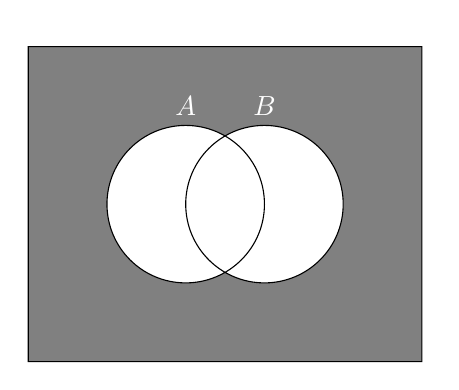
\begin{tikzpicture}[fill=gray]

        \begin{scope}
            \fill (-2,-2) rectangle (3,2);
        \end{scope}

        \begin{scope}
            \fill[white] (0,0) circle (1)
                         (1,0) circle (1);
        \end{scope}

        \draw (0,0) circle (1) (0,1)  node [text=white,above] {$A$}
              (1,0) circle (1) (1,1)  node [text=white,above] {$B$}
              (-2,-2) rectangle (3,2) node [text=black,above] {};
    \end{tikzpicture}

    \part

    \(\overline{A}\)
    \\

    \solution

    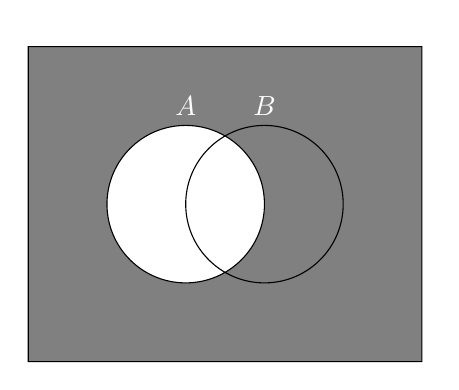
\begin{tikzpicture}[fill=gray]

        \begin{scope}
            \fill (-2,-2) rectangle (3,2);
        \end{scope}

        \begin{scope}
            \fill[white] (0,0) circle (1);
        \end{scope}

        \draw (0,0) circle (1) (0,1)  node [text=white,above] {$A$}
              (1,0) circle (1) (1,1)  node [text=white,above] {$B$}
              (-2,-2) rectangle (3,2) node [text=black,above] {};
    \end{tikzpicture}

    \pagebreak

    \part

    \(\overline{B}\)
    \\

    \solution

    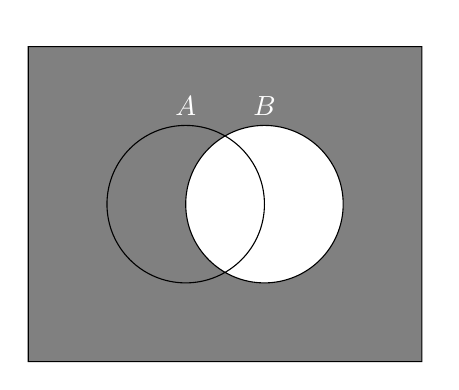
\begin{tikzpicture}[fill=gray]

        \begin{scope}
            \fill (-2,-2) rectangle (3,2);
        \end{scope}

        \begin{scope}
            \fill[white] (1,0) circle (1);
        \end{scope}

        \draw (0,0) circle (1) (0,1)  node [text=white,above] {$A$}
              (1,0) circle (1) (1,1)  node [text=white,above] {$B$}
              (-2,-2) rectangle (3,2) node [text=black,above] {};
    \end{tikzpicture}
    \\

    \part

    \(\overline{A} \cap \overline{B}\)
    \\

    \solution

    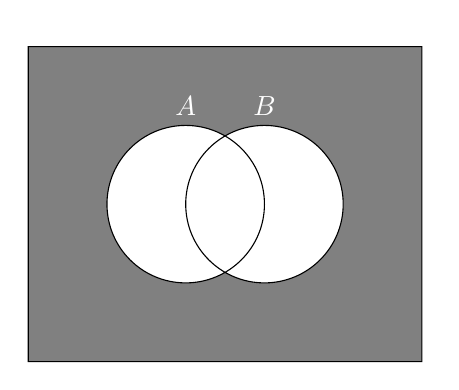
\begin{tikzpicture}[fill=gray]

        \begin{scope}
            \fill (-2,-2) rectangle (3,2);
        \end{scope}

        \begin{scope}
            \fill[white] (0,0) circle (1)
                         (1,0) circle (1);
        \end{scope}

        \draw (0,0) circle (1) (0,1)  node [text=white,above] {$A$}
              (1,0) circle (1) (1,1)  node [text=white,above] {$B$}
              (-2,-2) rectangle (3,2) node [text=black,above] {};
    \end{tikzpicture}

\end{homeworkProblem}

\end{document}
